\chapter{Metode Acuan}

\section{Latar Belakang Data}

Data yang digunakan adalah data pembacaan sensor pada pompa air yang berasal dari seorang pengguna di Kaggle \cite{pump_sensor_data}. Pompa air yang digunakan sering mengalami kerusakan sehingga menimbulkan permasalahan serius terhadap kehidupan warga. Tim yang bekerja tidak dapat melihat pola apapun pada data ketika sistem rusak, sehingga diharapkan dapat ditemukan suatu cara untuk memprediksinya.

\section{Data Preprocessing}

Data terdiri dari 220.320 entri yang terbagi dalam 3 grup utama:

\begin{enumerate}
    \item Timestamp
    \item Sensor
    \item Status mesin: Label target yang diprediksi ketika kerusakan akan terjadi
\end{enumerate}

Timestamp tertulis dalam format: \texttt{tahun-bulan-tanggal jam:menit:detik}

Sensor tersebar dalam 52 kolom dari \texttt{sensor\_00} hingga \texttt{sensor\_51} yang terdiri dari nilai float.

Status mesin terdiri dari 3 kelas: NORMAL, BROKEN, dan RECOVERING yang masing-masing menyatakan kondisi normal, rusak, dan pulih pada pompa.

    \subsection{Data Cleaning}

    Terdapat beberapa hal yang harus dilakukan terlebih dahulu pada data:

    \begin{enumerate}
        \item Menghapus kolom berlebih
        \item Menghapus duplikat
        \item Mengatasi nilai yang hilang (not available/NA)
        \item Mengkonversi tipe data ke tipe yang benar
    \end{enumerate}
    
    Untuk mengatasi nilai hilang dicari 10 sensor dengan jumlah NA terbanyak. Kemudian NA pada sensor tersebut diisi oleh nilai mean-nya (impute), sedangkan NA pada sensor lain dihapus.

    \subsection{Dimensional Reduction}

    Komputasi dengan seluruh kolom dari sensor akan membutuhkan waktu yang lama dan tidak efisien. Sehingga diterapkan principal component analysis (PCA) untuk menghasilkan fitur baru yang dapat digunakan pada modeling. Namun sebelum itu data perlu diskala terlebih dahulu karena PCA merupakan algoritma berbasis jarak. Jika dilihat pada 10 data pertama besar nilai bacaan tidak konsisten pada tiap sensor, beberapa sangat besar dan yang lain justru sangat kecil.

        \subsubsection{Principal Component Analysis}

        \begin{figure}[h]
            % \centering
            \centerline{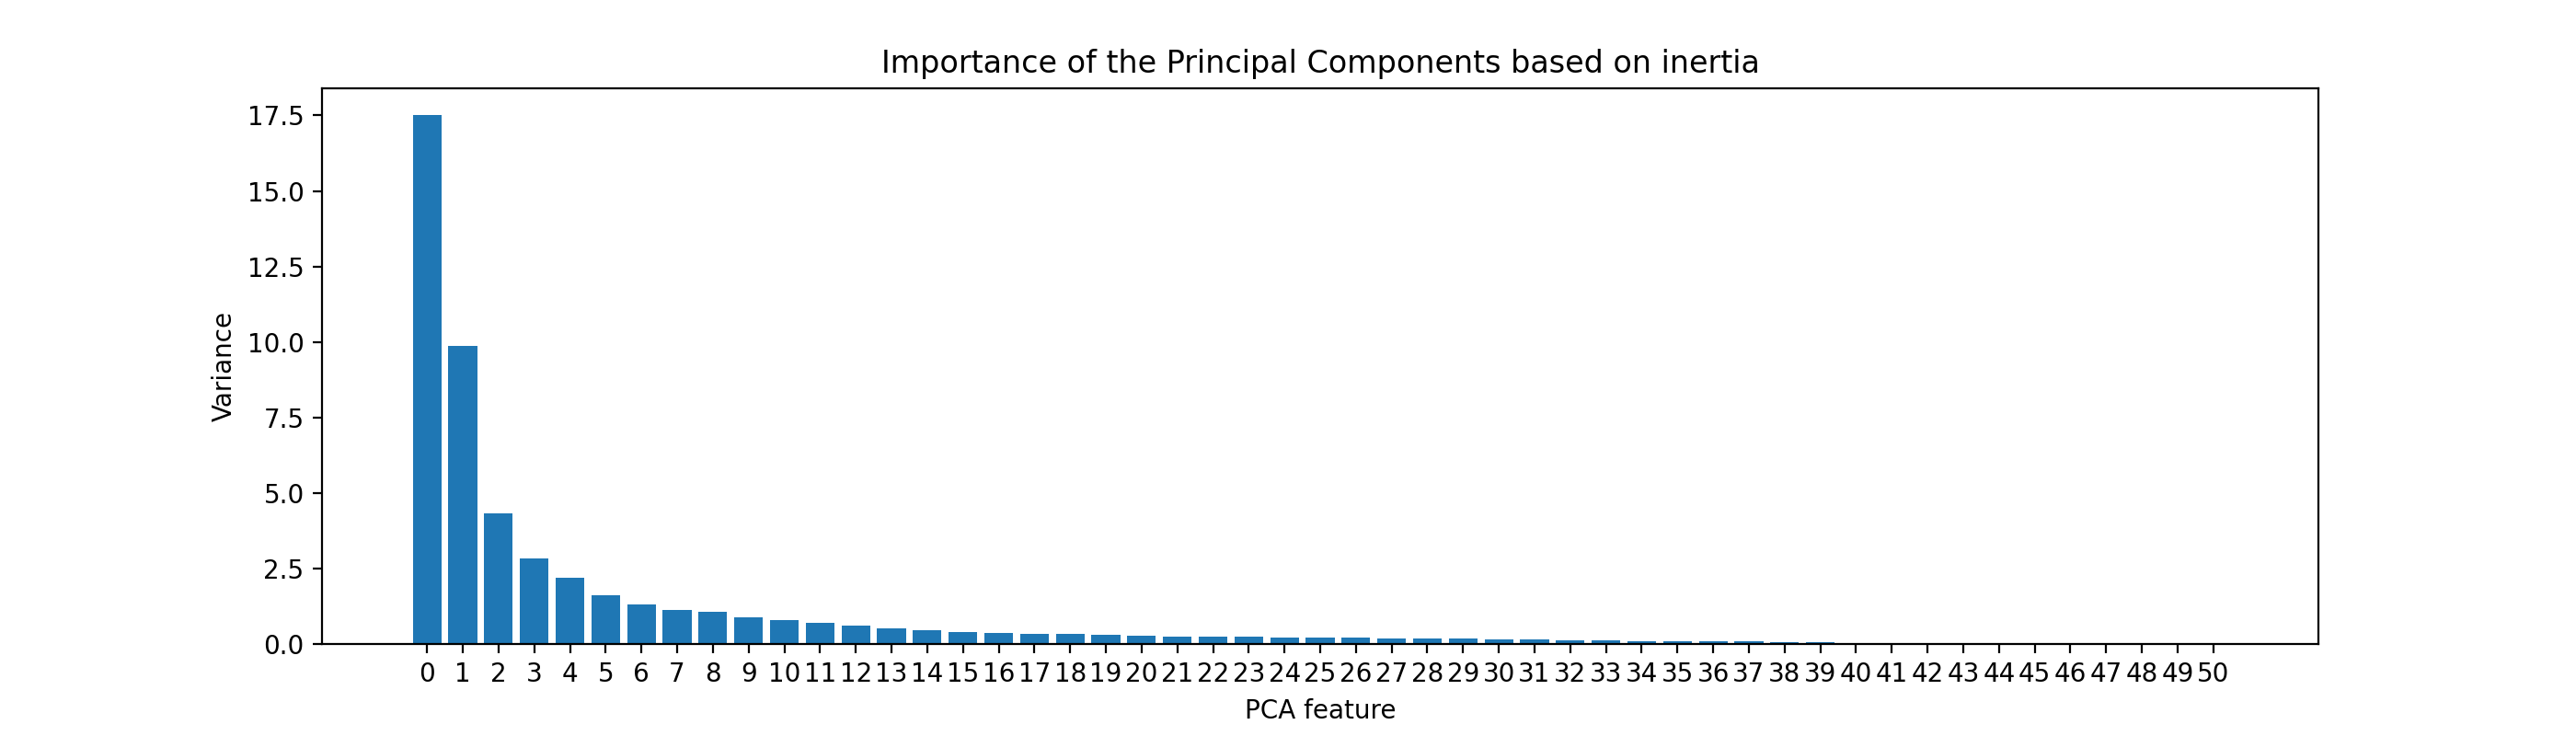
\includegraphics[width=1.2\textwidth]{resources/Acuan/PCA_Plot.png}}
            \caption{Komponen Utama PCA}
        \end{figure}

        Setelah dianalisis berdasarkan nilai variansi ternyata 2 komponen utama pertama adalah yang paling penting, sehingga PCA dilakukan dengan menggunakan 2 komponen tersebut yang kemudian digunakan pada pelatihan model.

        \subsubsection{Stationarity and Autocorrelation}

        Stationarity merupakan perilaku data time-series saat nilai mean dan standar deviasinya tidak berubah sepanjang waktu. Sedangkan autocorrelation merupakan perilaku data ketika terkorelasi dengan dirinya sendiri pada periode waktu yang berbeda.

        Untuk mengecek stationarity secara kuantitatif dilakukan Augmented Dickey-Fuller Test pada kedua komponen utama dari PCA.

\begin{python}
from statsmodels.tsa.stattools import adfuller
# Run Augmented Dickey Fuller Test
result = adfuller(principalDf['pc1'])
# Print p-value
print(result[1])
# Out : 5.453684941848713e-05

# Run Augmented Dickey Fuller Test
result = adfuller(principalDf['pc2'])
# Print p-value
print(result[1])
# Out : 1.8909142426286498e-06
\end{python}

        Untuk mengecek autocorrelation digunakan plot ACF (autocorrelation function) untuk memperoleh hasil secara visual.

\begin{python}
# Compute change in daily mean 
pca1 = principalDf['pc1'].pct_change()
# Compute autocorrelation
autocorrelation = pca1.dropna().autocorr()
print('Autocorrelation is: ', autocorrelation)
# Out : Autocorrelation is -0.002051194822378389

# Compute change in daily mean 
pca2 = principalDf['pc2'].pct_change()
# Compute autocorrelation
autocorrelation = pca2.autocorr()
print('Autocorrelation is: ', autocorrelation)
# Out : Autocorrelation is -3.150648347070906e-05
\end{python}

\section{Modeling}

    \subsection{Interquartile Range (IQR)}

    Strategi dari model ini adalah: \cite{metode_acuan}

    \begin{enumerate}
        \item Hitung nilai IQR, yaitu beda dari persentil ke-75 (Q3) dan ke-25 (Q1)
        \item Hitung batas atas dan bawah untuk outlier
        \item Filter data yang berada di atas dan di bawah batas dan tandai sebagai outlier
        \item Plot outlier di atas data time-series
    \end{enumerate}

\begin{python}
# Calculate IQR for the 1st principal component (pc1)
q1_pc1, q3_pc1 = df['pc1'].quantile([0.25, 0.75])
iqr_pc1 = q3_pc1 - q1_pc1

# Calculate upper and lower bounds for outlier for pc1
lower_pc1 = q1_pc1 - (1.5*iqr_pc1)
upper_pc1 = q3_pc1 + (1.5*iqr_pc1)

# Filter out the outliers from the pc1
df['anomaly_pc1'] = ((df['pc1']>upper_pc1) | \
    (df['pc1']<lower_pc1)).astype('int')

# Calculate IQR for the 2nd principal component (pc2)
q1_pc2, q3_pc2 = df['pc2'].quantile([0.25, 0.75])
iqr_pc2 = q3_pc2 - q1_pc2

# Calculate upper and lower bounds for outlier for pc2
lower_pc2 = q1_pc2 - (1.5*iqr_pc2)
upper_pc2 = q3_pc2 + (1.5*iqr_pc2)

# Filter out the outliers from the pc2
df['anomaly_pc2'] = ((df['pc2']>upper_pc2) | \
    (df['pc2']<lower_pc2)).astype('int')
\end{python}

    \subsection{K-Means Clustering}

    Strategi dari model ini adalah:

    \begin{enumerate}
        \item Hitung jarak antara tiap titik dan centroid terdekatnya. Jarak terbesar dianggap sebagai anomali.
        \item Gunakan parameter \texttt{outliers\_fraction} untuk memberi informasi pada algoritma tentang proporsi outlier yang ada pada data. Situasi dapat berbeda untuk tiap dataset. Namun sebagai langkah awal asumsikan \texttt{outliers\_fraction} = 0.13 (13\% dari data total adalah outlier).
        \item Hitung jumlah outlier dengan \texttt{outliers\_fraction}.
        \item Atur threshold sebagai jarak minimum dari outlier.
        \item Filter data dengan jarak lebih dari threshold sebagai anomali.
        \item Visualisasi anomali pada plot time-series.
    \end{enumerate}

\begin{python}
# Import necessary libraries
from sklearn.cluster import KMeans

# I will start k-means clustering with k=2 as I already
# know that there are 3 classes of "NORMAL" vs 

# "NOT NORMAL" which are combination of 
# BROKEN" and"RECOVERING"
kmeans = KMeans(n_clusters=2, random_state=42)
kmeans.fit(principalDf.values)
labels = kmeans.predict(principalDf.values)
unique_elements, counts_elements = \
    np.unique(labels, return_counts=True)
clusters = np.asarray((unique_elements, counts_elements))

# Write a function that calculates distance between each 
# point and the centroid of the closest cluster
def getDistanceByPoint(data, model):
    """ Function that calculates the distance between
     a point and centroid of a cluster, 
            returns the distances in pandas series"""
    distance = []
    for i in range(0,len(data)):
        Xa = np.array(data.loc[i])
        Xb = model.cluster_centers_[model.labels_[i]-1]
        distance.append(np.linalg.norm(Xa-Xb))
    return pd.Series(distance, index=data.index)

# Assume that 13% of the entire data set are anomalies 
outliers_fraction = 0.13

# get the distance between each point and its nearest 
# centroid. The biggest distances are considered as anomaly
distance = getDistanceByPoint(principalDf, kmeans)

# number of observations that equate to the 13% of 
# the entire data set
number_of_outliers = int(outliers_fraction*len(distance))

# Take the minimum of the largest 13% of the distances 
# as the threshold
threshold = distance.nlargest(number_of_outliers).min()

# anomaly1 contain the anomaly result of the above 
# method Cluster (0:normal, 1:anomaly) 
principalDf['anomaly1'] = (distance >= threshold).astype(int)
\end{python}

    \subsection{Isolation Forest}

    Model Isolation Forest ‘mengisolasi’ observasi dengan memilih fitur secara acak dan memilih nilai split antara nilai maksimum dan minimum untuk fitur terkait.

\begin{python}
# Import IsolationForest
from sklearn.ensemble import IsolationForest
# Assume that 13% of the entire data set are anomalies
    
outliers_fraction = 0.13
model =  IsolationForest(contamination=outliers_fraction)
model.fit(principalDf.values) 
principalDf['anomaly2'] = \
    pd.Series(model.predict(principalDf.values))
\end{python}

    \section{Evaluation}

    Dari ketiga model diperoleh jumlah data normal dan data anomali sebagai berikut.

    \begin{table}[h]
        \centering
        \begin{tabular}{|l|r|r|r|}
            \hline
            \multicolumn{1}{|c|}{\textbf{Metode}} & \multicolumn{1}{c|}{\textbf{Normal}} & \multicolumn{1}{c|}{\textbf{Anomali}} & \multicolumn{1}{c|}{\textbf{Persentase (\%)}} \\ \hline
            IQR                & 189.644 & 29.877 & 14 \\ \hline
            K-Means Clustering & 190.984 & 28.537 & 13 \\ \hline
            Isolation Forest   & 190.983 & 28.538 & 13 \\ \hline
        \end{tabular}
    \end{table}

\section{Modifikasi}
Beberapa modifikasi yang penulis lakukan pada kode acuan adalah
\begin{enumerate}
    \item Penyamaan format dan tampilan grafik
    \item Penambahan algoritma untuk menghitung kecepatan proses
    \item Penyesuaian statistika dari hasil prediksi model
\end{enumerate}